\chapter{Design}

V kapitole design popíšeme návrh realizace požadavků, které jsme popsali v kapitole analýza.

\section{Architektura aplikace}

Jako implementační jazyk jsme zvolili jazyk Java.

\subsection{Serverová část}

% TODO definice Cloudu
Serverová část aplikace poběží na serverech v Cloudu, to nám umožní efektivní správu prostředků, možnost trvalé expanze a škálovatelnost aplikace.
Pro volbu konkrétního poskytovatele jsme měli (v době zahájení práce) na výběr z:
\begin{itemize}
	\item Amazon EC2
	\item Google AppEngine
\end{itemize}

Jelikož jsme měli již zkušenost s druhým zmíněným a jeho architektura a API nám byla známá, zvolili jsme jej.

\subsubsection{Platforma Google AppEngine}

% TODO definice VPS
Google AppEngine je platforma pro vývoj a hostování webových aplikací psaných v jednom z několika podporovaných jazyků.
Poskytovatel účtuje jen prostředky skutečně využité, tím se liší od běžných VPS.
Platforma umožnuje automatické škálování výkonu podle aktuální potřeby aplikace.
Samotný výběr poskytovatele nám umožňuje splnit výkonostní požadavky.

AppEngine je platforma, která poskytuje několik spolu provázaných rozhraní.
Pro naši aplikaci jsou důležité především:
\begin{itemize}
	\item Datastore --- databáze pro uložení všech dat, jak sdílených, tak i dedikovaných jednotlivým uživatelům.
		Specifikem této databáze je, že formálně nemá schéma a má jen velice omezené možnosti dotazování na úkor výkonu.
		Mezi největší omezení patří nemožnost jakýchkoli spojení tabulek, veškeré filtry použité v dotazu mohou jen porovnávat hodnotu atributu s konstantou; toto omezení nutně ovlivnilo návrh entit a implementaci tříd.
		Dalším omezením je nutnost existence perfektního indexu pro každý dotaz, který se kdy bude provádět; neexistence indexu způsobí běhovou chybu.
		Na druhou stranu, nutnost zaindexování všech dotazů umožňuje extrémní rychlost databáze; každý dotaz se provádí ve dvou krocích:
		1. nalezení prvního výsledku v indexu; 2. výpis nalezeného záznamu a všech následujících, dokud záznam vyhovuje všem filtrům.
		Existují ještě další omezení, které nás příliš netrápí, například, že dotaz může vrátit neaktuální výsledky.
	\item Task Queue --- fronta úloh, skrze kterou projdou všechny úlohy.
		Fronta se stará o pravidelné spouštění úloh s pevnou frekvencí; to zajišťuje, že při kontrole zdrojů nedojde k většímu zatížení serveru.
		Kontrola každého zdroje je jedna úloha a fronta úloh se stará o to, aby bylo spuštěno jen určité množství úloh zároveň.
	\item Users --- ověřování uživatelů; aplikace přebírá údaje o aktuálně přihlášeném uživateli při každém požadavku.
		Nemusíme tedy řešit celou infrastrukturu kolem registrace, přihlašování, odhlašování, zapomenutého hesla.
	\item BlobStore a Files --- jelikož architektura serveru neumožňuje práci s filesystémem -- není známá informace o tom, na kterých serverech a kde na světě aplikace právě běží (potenciálně v několika instancích) -- posktuje server rozhraní ke své abstrakci souborů.
		My toto API použijeme k uložení a následné prezentaci zazálohovaných webových stránek článků.
\end{itemize}

\subsubsection{Úloha serverové části}

Serverová část bude mít v aplikaci následující úlohy:
\begin{itemize}
	\item uložení všech dat,
	\item poskytování dat klientům,
	\item periodický sběr nových položek kontrolou zdrojů,
	\item výpočet doporučení zdrojů klientům na základě podobnosti.
\end{itemize}

\subsubsection{Použité knihovny}

Abychom znovu nevynalézali kolo a neřešili problémy, které již jiní řešili před námi, použijeme několik knihoven, které nám zjednodušší implementaci vlatní aplikace.

\paragraph{Slim3}
% TODO link Slim3
Pro obalení nízkoúrovňového API pro přístup k databázi použijeme framework Slim3.
Slim3 zajišťuje mapování databázových bezschématických entit na reálné javové objekty.
Tento framework zároveň poskytuje objektově konzistentní rozhraní ke skládání databázových dotazů.
Tato knihovna je vyvinutá jen a pouze pro platformu AppEngine, neboť je silně závislá na Datastore API.

\paragraph{ROME}
%TODO link ROME
ROME je knihovna, která poskytuje sadu parserů a generátorů pro různé typy formátů zpravujících o novinkách na webovém zdroji.
My tuto knihovnu použijeme pro oba směry konverze, využijeme parsery při kontrole jednoho typu zdrojů a generátory při sdílení (exportu) položek.
ROME je starší knihovna, nezdá se, že by její vývoj pokračoval, nicméně je dostatečně robustní a stabilní pro naše potřeby.

\paragraph{Apache HttpComponents}
% TODO apache http components
% definice http
Apache HttpComponents je široce rozšířená knihovna uřcená pro zajištění komunikace přes HTTP.
My ji použijeme pro stahování webových dokumentů při kontrole zdrojů všech typů (kromě manuálního).

\paragraph{jsoup}
% TODO vysvětlit DOM
% TODO link jsoup
Knihovna jsoup umožňuje rozparsovat HTML stránku do DOM struktury a poskytuje metody na procházení a manipulaci se stromem elementů.
Knihovna zvládá zpracování i takových stránek, které nevyhovující standardům.
My knihovnu využijeme ve dvou situacích:
\begin{itemize}
	\item pro parsování webové stránky při kontrole některých typů zdrojů,
	\item pro úpravu relativních odkazů při zálohování webové stránky.
\end{itemize}

\paragraph{JScience}
% TODO link JScience
Knihovna JScience poskytuje implementaci nejrůznějších výpočetních algoritmů určených pro matematiku a fyziku.
Nás z této knihovny bude zajímat jen malá část: implementace vektorových a maticových operací, které použijeme při výpočtech doporučených zdrojů pro jednotlivé uživatele.

\paragraph{Diff Match Patch}
% TODO link diff match patch
Diff match patch je malá knihovna, která nabízí robustní algoritmy pro operace nutné při synchronizaci textu.
My využijeme jen jednu ze tří částí: porovnání dvou textů, které nám vrátí seznam rozdílů.

\subsection{Klientská část}

% TODO vysvětlit html, css, js
Klientská část apliakce je ta část, kterou si každý uživatel stáhne při návštěvě webové stránky aplikace.
Jelikož se aplikace spouští v internetovém prohlížeči, je omezená tamním prostředím: grafická část je tvořena jazykem HTML a CSS, výkonná část je napsána v jazyce JavaScript.
Jelikož serverová část aplikace je vytvořena v jazyce Java, zvolili jsme pro klientskou část nástroj, který umožňuje zkompilovat kód v jazyce Java do jazyku JavaScript, který je určen pro běh v prohlížeči.
Takovým nástrojem je Google Web Toolkit -- GWT; mezi jeho základní vlastnosti patří:
\begin{itemize}
	\item serverová i klientská část je psána ve stejném jazyce,
	\item společný kód pro serverovou a klientskou část se napíše jen jednou (a přeloží dvakrát),
	\item poskytuje základ pro komunikaci mezi klientskou a serverovou částí, stará se o serializaci a deserializaci požadavků,
	\item stará se o minifikaci kódu odeslaného klientovi,
	\item poskytuje hotové základní komponenty pro tvorbu uživatelského rozhraní.
\end{itemize}

\subsubsection{Úloha klientské části}

Klientská část je ta část aplikace, kterou uživatel ovládá pomocí prvků grafické prostředí webové stránky.
Skrze ní manipuluje se svými daty uloženými na serverové části aplikace.
Mezi nejdůležitější úkony prováděné uživatelem patří:
\begin{itemize}
	\item správa zdrojů: přidání a úprava zdroje, zatavení a obnovení sledování zdroje
	\item procházení seznamu položek, zobrazení originálu položky, přidání/odebrání štítku, zazálohování položky
	\item filtrování seznamu položek, změna kritérií filtru, správa filtrů
	\item nastavení ostatních vlastností aplikace
\end{itemize}

\subsubsection{Použité knihovny}

V klientské části aplikace použijeme jedinou knihovnu: GWT Eye Candy.
Tato knihovna nabízí kolekci ovládacich prvků do uživatelského prostředí aplikace.
My využijeme jen jediný prvek: ColorPicker pro výběr barvy štítků.

\subsection{Doplněk do prohlížeče}

% TODO link na crossrider
Využijeme služeb platformy Crossrider, která umožňuje vytvořit jeden doplněk, který bude fungovat stejně v nejrozšířenějších prohlížečích.
Podporované prohlížeče jsou:
% TODO link na FAQ 
\begin{itemize}
	\item Internet Explorer 7 a vyšší
	\item Chrome -- všechny verze
	\item Firefox -- 3.6 a vyšší
\end{itemize}

\subsubsection{Funkce doplňku}
% XXX Moc podrobně?

Doplněk slouží k přidání nové manuální položky do aplikace.
Doplněk bude mít podobu tlačítka na liště v prohlížeči; kliknutím na tlačítko se objeví vyskakovací okno s předvyplněnou adresou a titulkem aktuální stránky.
V připadě, že uživatel vybral kus textu na stránce, bude jím předvyplněn popis.
Kliknutím na tlačítko \uv{Odeslat} se vytvoří v aplikaci nová manuální položka podle vyplěných údajů.

\section{Entity}

Entity jsou obecné struktury, se kterými aplikace pracuje.
Cílem této kapitoly je entity popsat a vysvětlit úlohu, kterou hrají v kontextu celé aplikace.

\subsection{Oblast uživatele a konfigurace}

\subsubsection{Uživatel}

Uživatel je reprezentace osoby, která systém používá.
Entitu uživatele přebíráme od poskytovatele serveru pomocí Users API.

\subsubsection{Konfigurační položka}

Konfigurační položka nemá nic společného s termínem \textit{položka} and entitou položka.

Jedna konfigurační položka definuje jeden parametr, jak má aplikace vypadat nebo jak se má chovat; lze rozlišit dva typy konfiguračních položek:
\begin{itemize}
	\item konfigurace serverové části --- závisí na ní chování serverové části,
	\item konfigurace klientské části --- závisí na ní vzhled nebo chování klientské části.
		Hodnoty položek tohoto typu mohou záviset na konkrétním uživateli, který aplikaci používá.
\end{itemize}

\subsection{Oblast zdrojů}

Tato část seskupuje všechny entity, které jsou souvisí se zdroji položek, jejich reprezentací a zpracováním.
Nejdůležitější dvojicí entit je zdroj a uživatelský zdroj: první má význam pouze pro pravidelné kontroly exitence nových položek, druhá popisuje zdroj z pohledu uživatele.

\subsubsection{Zdroj}

Zdroj reprezentuje každou webovou stránku nebo službu, kterou aplikace používá k získávání nových položek.
Aplikace pravidelně kontroluje změny na zdrojích; pokud ke změně dojde, aplikace přidá odpovídající položky.
Zdroj je abstraktní entita, od které jsou odvozeny jednotlivé typy zdrojů; obsahuje všechny informace nutné k tomu, aby zdroj mohl být periodicky kontrolován.

\paragraph{Manuální zdroj}

Manuální zdroj patří vždy jednomu uživateli.
Nereprezentuje žádnou internetovou adresu a sám o sobě neposkytuje žádné položky.
Všechny položky, které tomuto zdroji patří, přidal sám uživatel skrze jednu ze služeb k tomu určených.

\paragraph{RSS/Atom}

RSS a Atom jsou formáty XML dokumentů, které popisují novinky, ke kterým došlo za poslední dobu na webovém portálu.
Tento zdroj typicky obsahuje odkazy na články, které byly publikovány v nedávné minulosti.

\paragraph{Webový rozcestník}

Nahrazuje funkcionalitu RSS či Atom pro webové portály, které tyto kanály neposkytují.
Vychází z jednoduchého pozorování, že úvodní stránka takového portálu obsahuje seznam nedávných článků a že položky převzaté z RSS či Atomu by odpovídaly odkazům na této stránce.

\paragraph{Změna stránky}

Reprezentuje webovu stránku o jejíž změně obsahu chce uživatel být informován.
Každá změna stránky způsobí vytvoření položky informující o změně.

\subsubsection{Region}

Pro typ zdroje Webový rozcestník a Změna stránky definuje oblast stránky, jež je z pohledu uživatele zajímavá.
Oblast na stránce je určena výběrem oblastí stránky, které se mají kontrolovat a oblastí, které se mají při kontrole ignorovat.
Motivací k pozitivnímu a negativnímu přístupu k jednotlivým částem je fakt, že stránky obsahují obsah, který se mění při každém dotazu (reklamy, informace o času generování stránky) nebo není zajímavý (hlavička a patička stránky, menu).

\subsubsection{Uživatelský zdroj}

Entita zdroj slouží výhradně pro účely periodické kontroly, proto zavedeme entitu uživatelský zdroj, jež realizuje vztah mezi uživateli a zdroji.
Několik uživatelů může sledovat ten samý zdroj a každý uživatel většinou sleduje více zdrojů.
Zároveň tato entita uchovává vlastní nastavení každého zdroje zvlášť pro každého uživatele.
Počet aktivních uživatelských zdrojů určuje, zda o zdroj je zájem a jestli má probíhat jeho kontrola.
Pokud je v uživatelském rozhraní zmíněn pojem zdroj, je jím myšlena tato entita; entita zdroje nemá pro uživatele praktický význam.

\subsection{Oblast položek}

\subsubsection{Položka}

Položkou v aplikaci myslíme jednu adresu webové stránky, která pochází z některého ze zdrojů nebo byla přidána uživatelem manuálně.
Položka je závislá jen na zdroji, ze kterého pochází, vlastní personalizaci (přizpůsobení jednotlivým uživatelům) má na starosti entita uživatelská položka.
Každý typ zdroje poskytuje položky jiného typu:

\paragraph{Manuální položka}

Manuální položka formálně patří k manuálnímu zdroji; jediným důvodem je zajištění konzistence rozhraní všech typů položek.
Manuální položka reprezentuje libovolnou internetovou adresu spolu s titulkem a popisem.
Manuální položka vzniká jen a pouze činností uživatele, který si ji sám přidá do aplikace.
Motivací zavést manuální položku je umožnění uživateli:
\begin{itemize}
	\item přidat informaci k libovolné stránce,
	\item zazálohovat libovolnou stránku,
	\item označit si libovolnou stránku k pozdějšímu přečtení.
\end{itemize}

\paragraph{Položka typu článek}

Položka typu článek je produkována zdrojem RSS/Atom.
Každému záznamu v XML dokumentu odpovídá jedna položka vytvořená v aplikaci při kontrole zdroje.
Titulek a popis přebíráme spolu s dalšími informacemi přímo z RSS/Atom dokumentu.
Položek typu článek může poskytovat více informací než jiné typy položek: jedná se především o jméno autora článku a datum publikace.
Tyto informace není obecně možné jednoduše zjistit v případě položek jiných typů.

\paragraph{Položka typu odkaz}

Položka typu odkaz pochází ze zdroje typu webový rozcestník.
Každému nalezenému odkazu na webové stránce (uvnitř regionem omezené oblasti) odpovídá přavě jediná položka.
Titulek resp. popis přebíráme z textu odkazu reps. textu nejbližšího okolí odkazu.

\paragraph{Položka typu změna stránky}

Položka typu změna stránky pochází ze zdroje typu změna stránky.
Při kontroly stránky (na kterou se odkázuje zdroj) se porovnává její textový obsah s verzí, kterou jsme si uložili při předchozí kontrole.
Pokud je nalezena změna, aplikace vytvoří novou položku, která bude obsahovat popis změn stránky.

\bigskip{}

Položka je závislá jen na zdroji, ze kterého pochází; stejně jako v oblasti zdrojů existuje dvojice: zdroj -- uživatelský zdroj, existuje i entita uživatelská položka.

\subsubsection{Uživatelská položka}

Entita položka obsahuje jen obecné --- na uživateli nezávislé atributy, které jsou sdíleny všemi uživateli.
Jsou jimi například: titulek, obsah, zdroj, ze kterého pochází, datum a čas přidání.
Aby mohl každý uživatel mít položku ve vlastním stavu, s vlastními štítky, zavedeme entitu uživatelská položka.
Tato entita uchovává vlastní nastavení zvlášť pro každého uživatele.
Pokud je v uživatelském rozhraní zmíněn pojem položka, je jím myšlena tato entita; entita položka nemá pro uživatele praktický význam.

\bigskip{}

Na obrázku \ref{fig:source-item} je zobrazen vztah nejdůležitějších entit z oblastí zdrojů a položek.

\begin{figure}
    \centering
    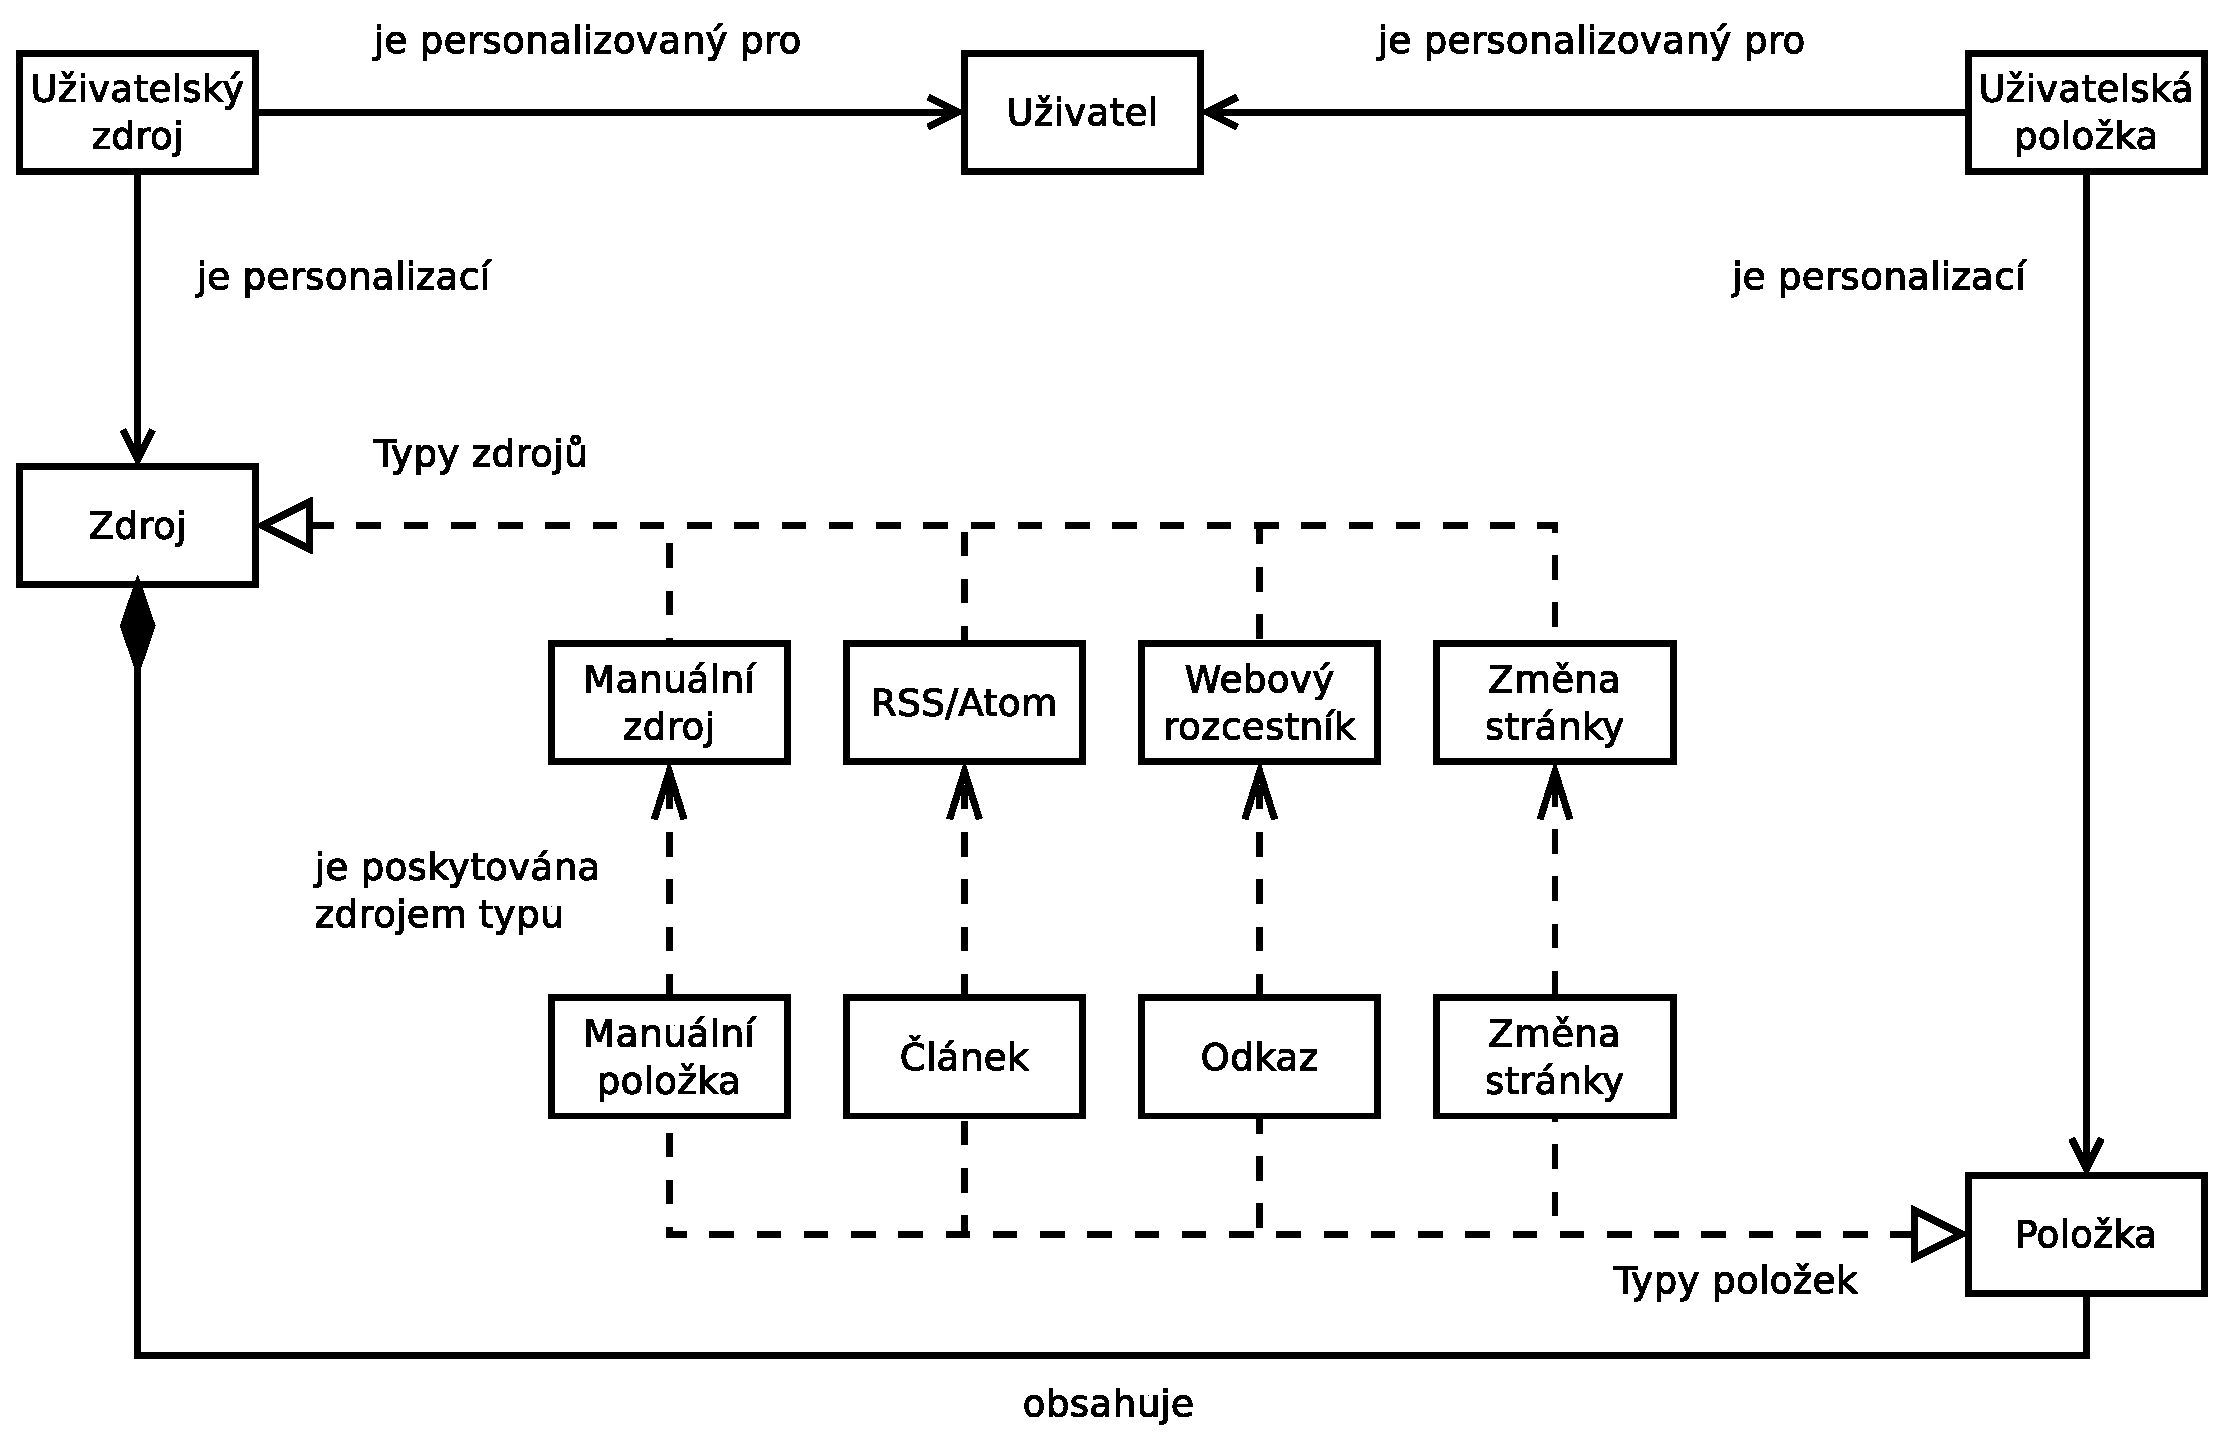
\includegraphics[width=12cm]{img/zdroje-polozky.eps}
    \caption{Vztahy mezi uživatelem, zdroji a položkami}
    \label{fig:source-item}
\end{figure}

\subsection{Oblast štítků}

\section{Rozhraní pro komunikaci klienta se serverem}

\section{Procesy}

\section{Sběr položek}

\section{Doporučování}
